\documentclass[border=10pt]{standalone}

\usepackage{tikz}
\usepackage{tikzsymbols}
\usetikzlibrary{calc,patterns,shapes.geometric}

\def\centerarc[#1](#2)(#3:#4:#5){\draw[#1] ($(#2)+({#5*cos(#3)},{#5*sin(#3)})$) arc (#3:#4:#5);}

\begin{document}
	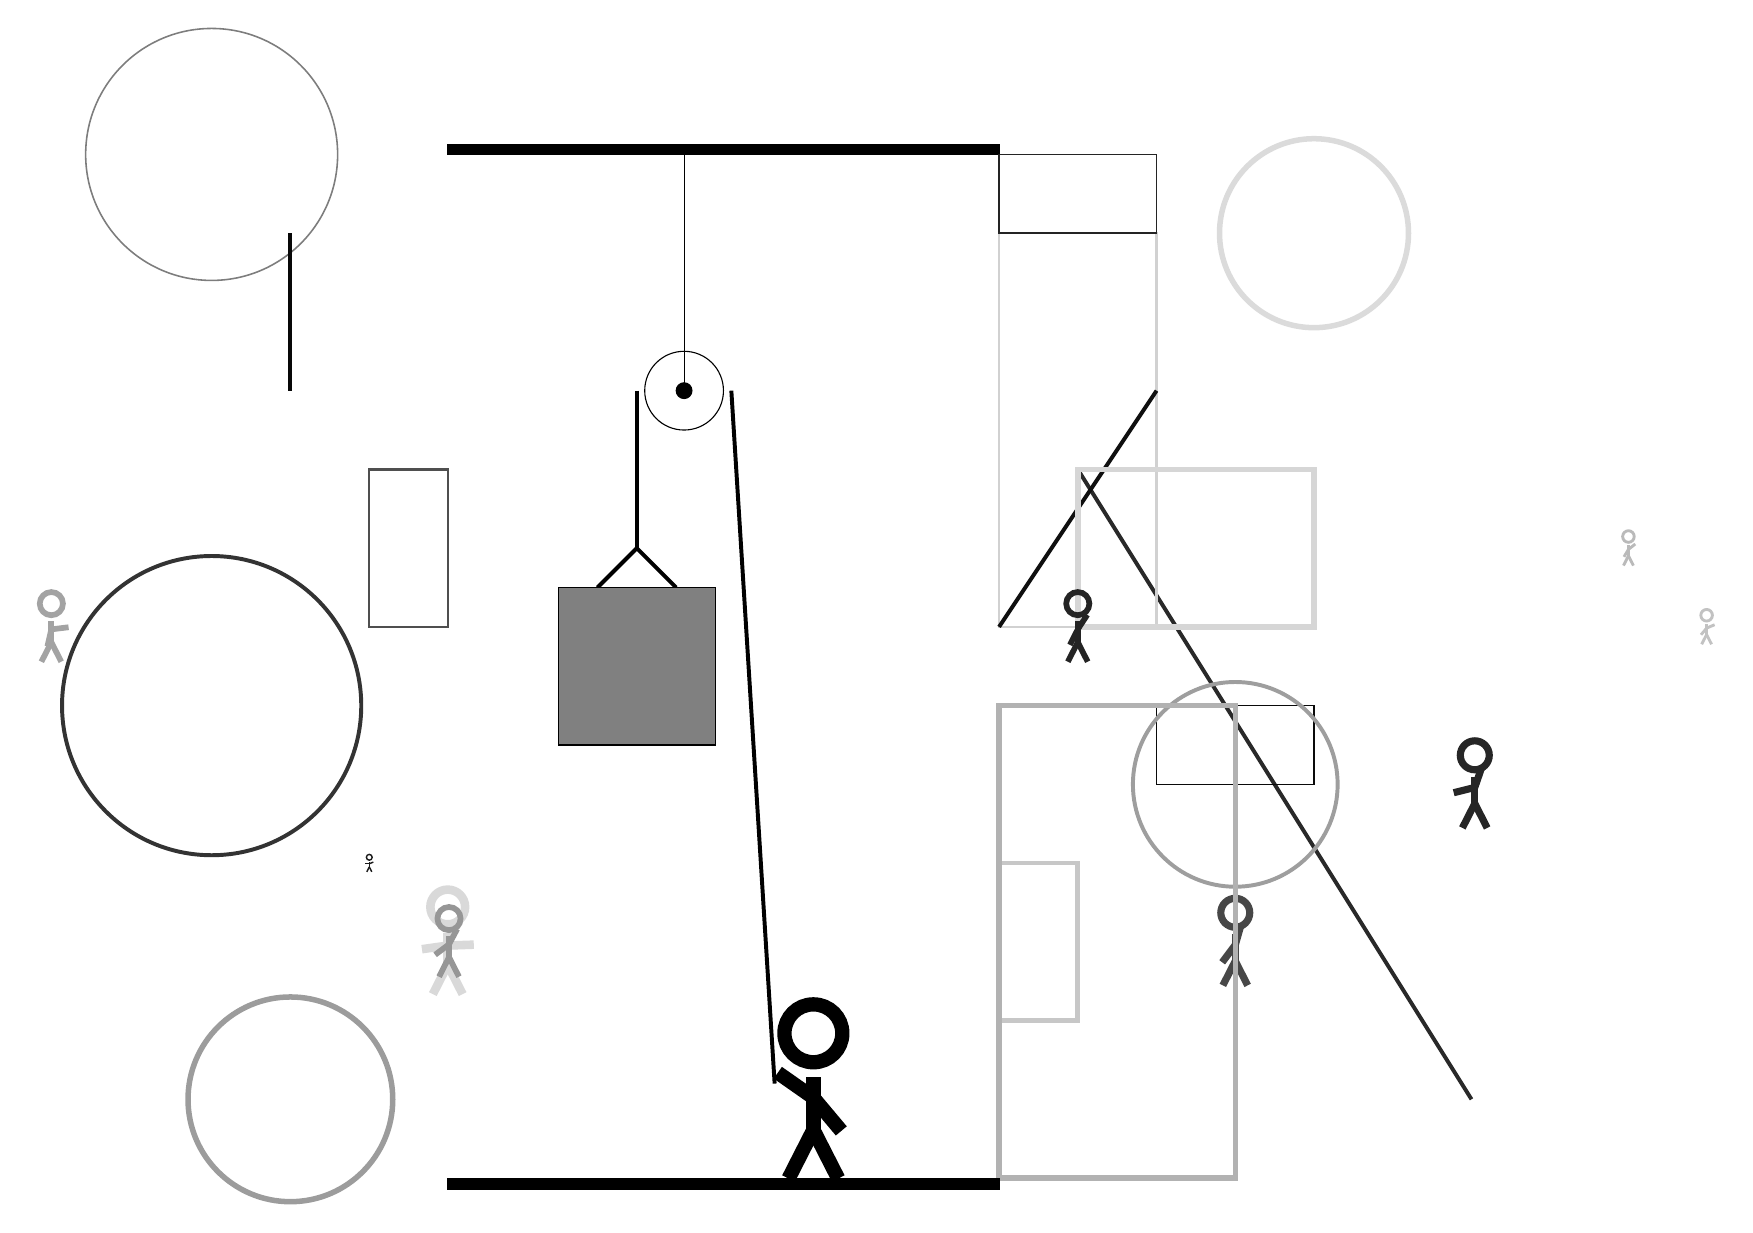
\begin{tikzpicture}
		%%%%% START %%%%%
		
		\draw[fill=black] (-2, 10) rectangle (5, 10.125);
		
		\draw (1, 7) circle (0.5);
		\draw[fill=black] (1, 7) circle (0.1);
		\draw (1, 10) -- (1, 7);
		
		\draw[line width=0.5mm] (-0.1, 4.5) -- (0.4, 5.0) -- (0.9, 4.5);
		\draw[fill=black!50] (-0.6, 4.5) rectangle (1.4, 2.5);
		
		\draw[line width=0.5mm] (0.4, 7) -- (0.4, 5.0);
		\centerarc[line width=0.5mm](1, 7)(0:180:0.6);
		\draw[line width=0.5mm](1.6, 7) -- (2.15, -1.8);
		
		\draw [line width=0.5mm, color=black!80](-5, 3) circle (1.9);
		
		\draw[line width=0.5mm, color=black!17](5, 8) -- (5, 8);
		\draw [line width=0.7mm, color=black!39](-4, -2) circle (1.3);
		\draw[line width=0.5mm, color=black!84](6, 6) -- (11, -2);
		\node[line width=0.5mm, color=black!85] at (11, 2) {\Strichmaxerl[5][14][71]};
		
		\draw[line width=0.3mm, color=black!69] (-2, 6) rectangle (-3, 4);
		\node[line width=0.6mm, color=black!36] at (-7, 4) {\Strichmaxerl[4][77][7]};
		
		\node[line width=0.2mm, color=black!15] at (-2, 0) {\Strichmaxerl[6][8][2]};
		\draw [line width=0.2mm, color=black!51](-5, 10) circle (1.6);
		
		\draw[line width=0.2mm, color=black!96] (7, 2) rectangle (9, 3);
		
		\node[line width=0.5mm, color=black!72] at (8, 0) {\Strichmaxerl[5][53][74]};
		\draw [line width=0.7mm, color=black!14](9, 9) circle (1.2);
		\draw[line width=0.3mm, color=black!18] (5, 4) rectangle (7, 9);
		
		\draw[line width=0.5mm, color=black!94](5, 4) -- (7, 7);
		\draw[line width=0.6mm, color=black!22] (5, 1) rectangle (6, -1);
		\draw[line width=0.7mm, color=black!16] (6, 4) rectangle (9, 6);
		\draw[line width=0.5mm, color=black!97](-4, 9) -- (-4, 7);
		\draw [line width=0.5mm, color=black!38](8, 2) circle (1.3);
		\node[line width=0.4mm, color=black!41] at (-2, 0) {\Strichmaxerl[4][37][62]};
		\draw[line width=0.2mm, color=black!86] (5, 9) rectangle (7, 10);
		\draw[line width=0.7mm, color=black!30] (5, -3) rectangle (8, 3);
		
		\node[line width=0.5mm, color=black!27] at (13, 5) {\Strichmaxerl[2][59][38]};
		\node[line width=0.5mm, color=black!89] at (-3, 1) {\Strichmaxerl[1][0][22]};
		\node[line width=0.7mm, color=black!86] at (6, 4) {\Strichmaxerl[4][63][57]};
		\node[line width=0.3mm, color=black!24] at (14, 4) {\Strichmaxerl[2][50][23]};
		
		\node at (2.6, -1.9) {\Strichmaxerl[10][-35][-50]};
		
		\draw[fill=black] (-2, -3) rectangle (5, -3.15);
		
		%%%%% END %%%%%
	\end{tikzpicture}
\end{document}